\subsection{Caso d'uso UC10: Modalità allenamento}
\begin{center}
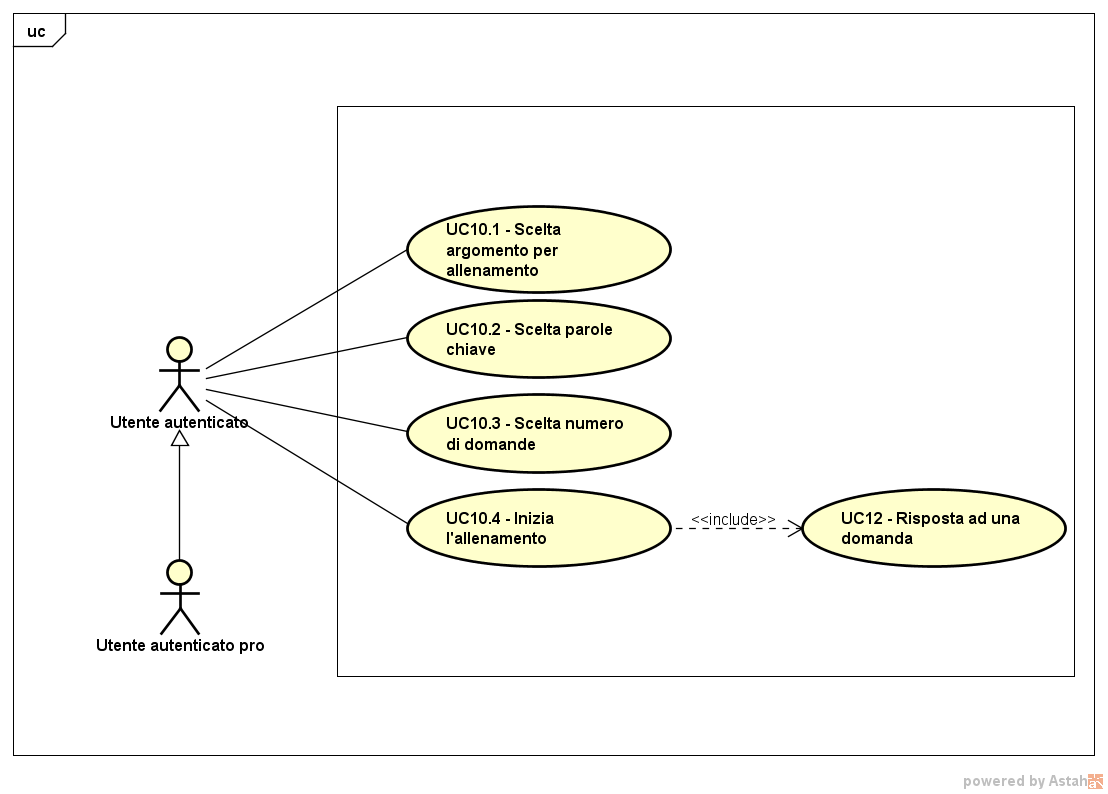
\includegraphics[scale=0.5]{UML/UC10.png}
\end{center}
\begin{itemize}
\item\textbf{Attori}: Utente autenticato, Utente autenticato pro;
\item\textbf{Descrizione}: l'utente autenticato/autenticato pro può svolgere un allenamento che consiste nel rispondere a domande che gli vengono proposte in modo dinamico. Ogni domanda può incrementare o decrementare il punteggio dell'allenamento per fare in modo che la difficoltà delle domande proposte sia sempre in linea con la competenza dell'utente sull'argomento scelto;
\item\textbf{Precondizione}: l'utente autenticato/autenticato pro ha selezionato l'opzione di allenamento;
\item\textbf{Postcondizione}: l'utente ha finito di svolgere l'allenamento e può quindi visualizzare la valutazione finale che ha ottenuto e il riepilogo delle risposte date nonchè il proprio livello sugli argomenti;
\item\textbf{Scenario principale}:
	\begin{itemize}
		\item L'utente autenticato/autenticato pro sceglie l'argomento per iniziare l'allenamento (UC10.1);
		\item L'utente autenticato/autenticato pro sceglie delle parole chiave (UC10.2);
		\item L'utente autenticato/autenticato pro sceglie il numero di domande che compongono l'allenamento (UC10.3);
	\end{itemize}
\item \textbf{Inclusione}:
	\begin{itemize}
		\item L'utente autenticato/autenticato pro inizia l'allenamento (UC12);
	\end{itemize}
\end{itemize}

\subsubsection{Caso d'uso UC10.1: scelta argomento per l'allenamento}
	\begin{itemize}
		\item \textbf{Attori}: Utente autenticato, Utente autenticato pro;
		\item \textbf{Descrizione}: Gli attori scelgono un macro argomento per eseguire un allenamento;
		\item \textbf{Precondizione}: Gli attori scelgono di eseguire un allenamento;
		\item \textbf{Postcondizione}: Gli attori hanno scelto un macro argomento per l'allenamento.
	\end{itemize}
\subsubsection{Caso d'uso UC10.2: scelta parole chiave}
	\begin{itemize}
		\item \textbf{Attori}: Utente autenticato, Utente autenticato pro;
		\item \textbf{Descrizione}: Gli attori scelgono delle parole chiave per filtrare in modo più dettagliato possibile l'argomento delle domande proposte per l'allenamento;
		\item \textbf{Precondizione}: Gli attori hanno scelto un argomento;
		\item \textbf{Postcondizione}: Gli attori hanno scelto delle parole chiavi.
	\end{itemize}
\subsubsection{Caso d'uso UC10.3: scelta numero di domande}
	\begin{itemize}
		\item \textbf{Attori}: Utente autenticato, Utente autenticato pro;
		\item \textbf{Descrizione}: Gli attori scelgono il numero di domande che comporranno l'allenamento, senza restrizione sul numero e ipoteticamente anche infinito;
		\item \textbf{Precondizione}: Gli attori hanno scelto un argomento e scelto delle parole chiavi;
		\item \textbf{Postcondizione}: Gli attori hanno scelto il numero di domande che comporranno l'allenamento.
	\end{itemize}
\subsubsection{Caso d'uso UC10.4.1: conferma risposta}
	\begin{itemize}
		\item \textbf{Attori}: Utente autenticato, Utente autenticato pro;
		\item \textbf{Descrizione}: Gli attori confermano la risposta data;
		\item \textbf{Precondizione}: Gli attori hanno risposto ad una domanda;
		\item \textbf{Postcondizione}: Gli attori hanno confermato la risposta e porseguono l'allenamento.
	\end{itemize}
\subsubsection{Caso d'uso UC10.4.2: like alla domanda}
	\begin{itemize}
		\item \textbf{Attori}: Utente autenticato, Utente autenticato pro;
		\item \textbf{Descrizione}: Gli attori possono lasciare un like a una domanda proposta;
		\item \textbf{Precondizione}: Agli attori è stata proposta una domanda;
		\item \textbf{Postcondizione}: Gli attori hanno rilasciato un like alla domanda proposta;
	\end{itemize}
\subsubsection{Caso d'uso UC10.4.3: commenti alla domanda}
	\begin{itemize}
		\item \textbf{Attori}: Utente autenticato, Utente autenticato pro;
		\item \textbf{Descrizione}: Gli attori possono scegliere di commentare una domanda;
		\item \textbf{Precondizione}: Gli attori hanno risposto ad una domanda e visualizzano una sezione per i commenti;
		\item \textbf{Postcondizione}: Gli attori hanno scelto di commentare la domanda proposta;
	\end{itemize}
\subsubsection{Caso d'uso UC10.4.3.1: scrivi commento}
	\begin{itemize}
		\item \textbf{Attori}: Utente autenticato, Utente autenticato pro;
		\item \textbf{Descrizione}: Gli attori possono scrivere il commento alla domanda proposta;
		\item \textbf{Precondizione}: Gli attori hanno scelto di scrivere un commento;
		\item \textbf{Postcondizione}: Gli attori hanno commentato la domanda proposta.
	\end{itemize}
\subsubsection{Caso d'uso UC10.4.4: segnalare la domanda}
	\begin{itemize}
		\item \textbf{Attori}: Utente autenticato, Utente autenticato pro;
		\item \textbf{Descrizione}: Gli attori possono segnalare una domanda se ritengono che sia sbagliata, mal formata oppure contenga contenuti non appropiati;
		\item \textbf{Precondizione}: Gli attori hanno visualizzato il resoconto dell'allenamento;
		\item \textbf{Postcondizione}: Gli attori hanno scelto di segnalare una domanda;
	\end{itemize}
\subsubsection{Caso d'uso UC10.4.5: scrivi segnalazione}
	\begin{itemize}
		\item \textbf{Attori}: Utente autenticato, Utente autenticato pro;
		\item \textbf{Descrizione}: Gli attori posso scrivere un commento sulla segnalazione per approfondire la motivazione;
		\item \textbf{Precondizione}: Gli attori hanno scelto di segnalare una domanda;
		\item \textbf{Postcondizione}: Gli attori hanno segnalato una domanda;
	\end{itemize}
\subsubsection{Caso d'uso UC10.4.6: avanzamento domanda successiva}
	\begin{itemize}
		\item \textbf{Attori}: Utente autenticato, Utente autenticato pro;
		\item \textbf{Descrizione}: Gli attori possono avanzare alla domanda successiva dopo aver risposto alla domanda proposta; 
		\item \textbf{Precondizione}: Gli attori hanno risposto alla domanda proposta;
		\item \textbf{Postcondizione}: Gli attori visualizzano la domanda sucessiva;
	\end{itemize}
\subsubsection{Caso d'uso UC10.4.7: conclusione allenamento e visualizzazione del risultato finale}
	\begin{itemize}
		\item \textbf{Attori}: Utente autenticato, Utente autenticato pro;
		\item \textbf{Descrizione}: Gli attori possono concludere l'allenamento in qualunque punto dell'allenamento;
		\item \textbf{Precondizione}: Gli attori stanno eseguendo un allenamento;
		\item \textbf{Postcondizione}: Gli attori hanno concluso l'allenamento;
	\end{itemize}
